\begin{figure}[htbp]
\centering
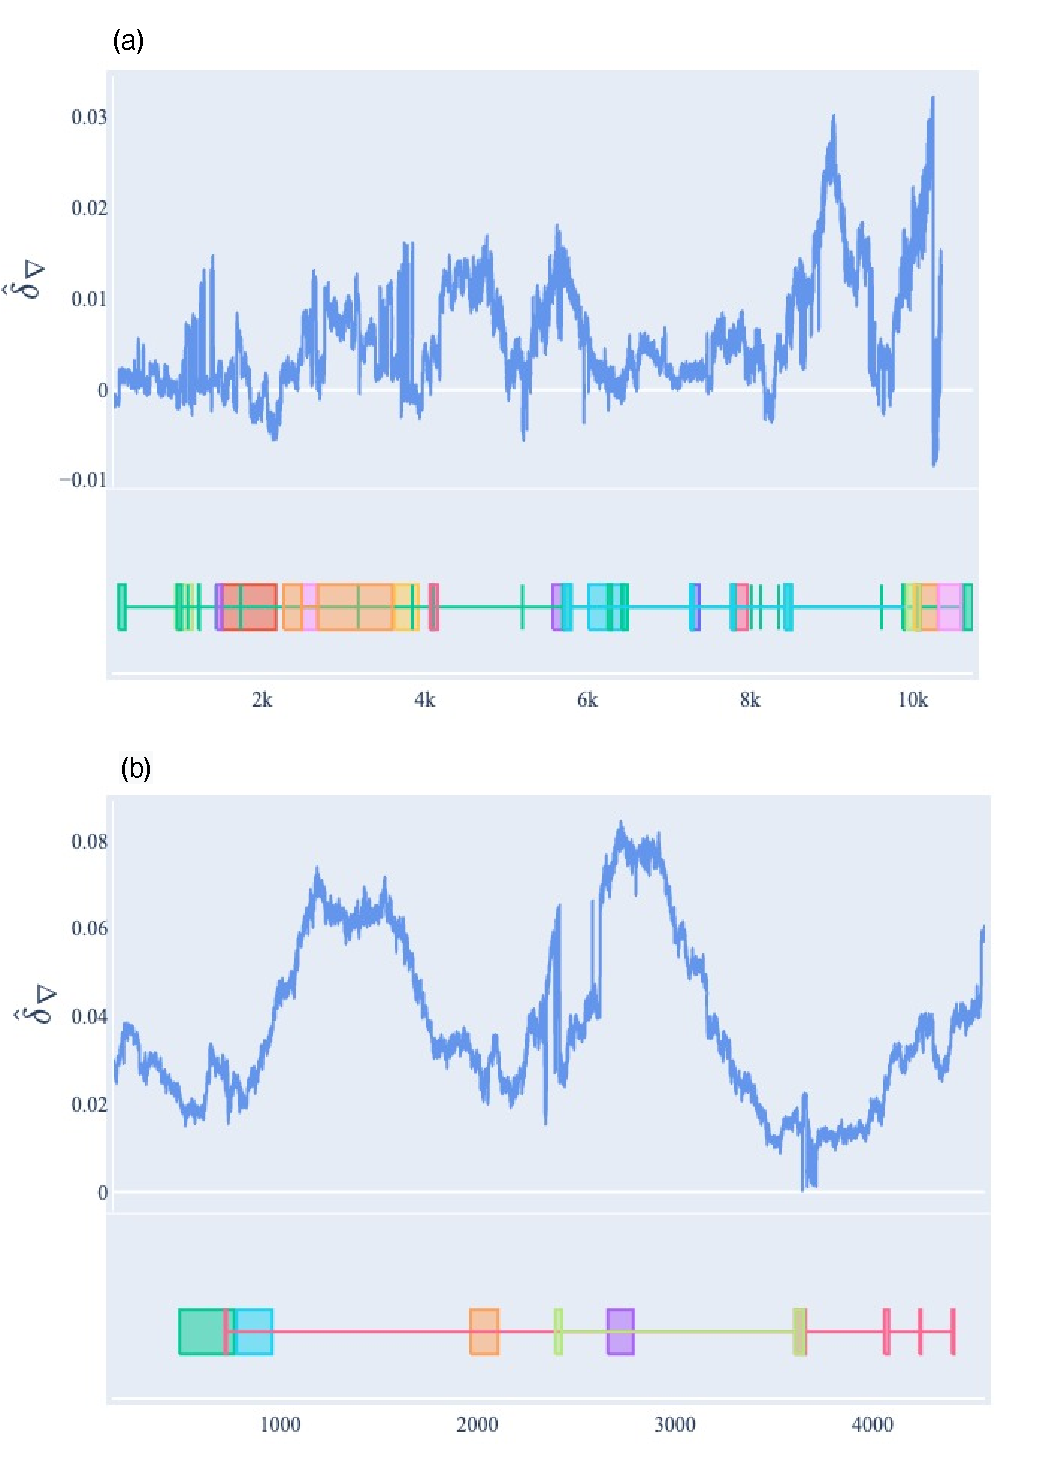
\includegraphics[width=0.9\textwidth]{figures/plots/rodent/dconv-intron3_4.pdf}
\caption{\textbf{Moving average of $\hat\delta_\nabla$ within \textit{Fxy} introns.}
\textbf{(a)}, intron 3, \textbf{(b)}, intron 4. The scatter plot shows the position of the mid point of a `sliding window' across the intron against the smoothed moving average of $\hat\delta_\nabla$. The location of annotated repeats in the \textit{M. musculus} sequence are indicated with the segments at the bottom of the figure. Different colours simply indicate different classes of repeats. The window looked at 600 positions of the raw alignment, and calculated $\hat\delta_\nabla$ if more than 300 positions remained after filtering. The taxa included in the alignment were \textit{M. musculus}, \textit{M. spretus}, and \textit{R. norvegicus}. In all model fitting \textit{M. musculus} was considered the foreground edge. }
\label{fig:rodent/d-conv/intron3_4}
\end{figure}